%\documentclass[10pt,handout]{beamer}
\documentclass[10pt]{beamer}
\usepackage[english]{babel} % Anpassa efter svenska. Ger svensk logga.
\usepackage[utf8]{inputenc} % Anpassa efter linux
\usepackage{graphicx}
\usetheme{Uppsala}
%\usecolortheme{UU} % Anpassa efter UU:s frger och logga
%\hypersetup{pdfpagemode=FullScreen} % Adobe Reader ska ppna fullskrm
\setbeamertemplate{itemize items}[circle]

% \usepackage{beamerthemesplit}
\usepackage{amsmath}
\usepackage{amssymb}
% \usepackage{graphics}
% \usepackage{graphicx}
% \usepackage{epsfig}
% \usepackage[latin1]{inputenc}
 \usepackage{color}
% \usepackage{fancybox}
% \usepackage{psfrag}
% \usepackage[english]{babel}
 \setbeamertemplate{footline}{\hfill\insertframenumber/\inserttotalframenumber}

%library(tinytex)
%tlmgr_install('booktabs')
\usepackage{booktabs}

%library(tinytex)
%tlmgr_install('csquotes')
\usepackage{csquotes}

%\usepackage{bm}
%\usepackage{natbib}
\newcommand{\bfm}[1]   {\mbox{\boldmath{${#1}$}}}
\newcommand{\Prob}   {\mbox{\textnormal{P}}}
\def\eqd{\,{\buildrel d \over =}\,}
\DeclareMathOperator{\E}{\mathbb{E}}

%%%%%%%%%%%%%%%%%%%%%%%%%%%%%%%%%%%%%%%%%%%%%%%%%%%%%%%%%%%%%%%%%%

\setlength{\parskip}{3mm}
\title[]{{\color{black}Machine learning, big data and artificial intelligence -- Block 8}}
\author[]{M{\aa}ns Magnusson\\Department of Statistics, Uppsala University}
\date{HT 2021}


\begin{document}

\frame{\titlepage
% \thispagestyle{empty}
}


\section{Previous assignments}

\begin{frame}{Practicalities}

\begin{itemize}
\item New exercise sessions: Dec 22, Dec 29, Jan 3, and Jan 5 on Zoom:
\texttt{https://uu-se.zoom.us/my/andreasostling}
\end{itemize}

\end{frame}

\begin{frame}{Assignment 5}

\begin{itemize}
\item MNIST vs. IMDB: Bias, variance or Bayes Error?
\end{itemize}

\end{frame}

\begin{frame}{Assignment 6: Evaluation}

\begin{itemize}
\item The Deep Learning book is hard to understand? How improve?
\item Clarifying as we go.
\item Long time of putting together the report? How can we make this simpler?
\end{itemize}

\end{frame}

%%%%%%%%%%%%%%%%%%%%%%%%%%%%%%%%%%%%%%%%%%%%%%%%%%%%%%%%%%%%%%%%%%


\begin{frame}{This week's lectures}
\begin{itemize}
\item Variational autoencoders
\item Probabilistic Topic Models
\end{itemize}
\end{frame}


%%%%%%%%%%%%%%%%%%%%%%%%%%%%%%%%%%%%%%%%%%%%%%%%%%%%%%%%%%%%%%%%%%


\begin{frame}{Why variational autoencoders and topic models?}
\begin{itemize}
\item Popular approaches in {\color{uured}industry and academia}
\item {\color{uured}Probabilistic} methods for unsupervised learning\pause
\item {\color{uured}Aim} of this lecture:
\begin{itemize}
\item Describe the models
\item How to estimate these models
\item Explain what they are used for
\end{itemize}
\end{itemize}
\end{frame}

\begin{frame}{Use Cases}

\begin{itemize}
\item Variational autoencoders: Unsupervised modeling of {\color{uured}images}
\item Topic models: Unsupervised modeling of {\color{uured}documents}
\end{itemize}

\pause

\begin{itemize}
\item Used for:
\begin{itemize}
\item Identify "{\color{uured}closeness}" in high-dimensional data\pause
\item {\color{uured}Visualize} data\pause
\item {\color{uured}Compression}\pause
\item {\color{uured}Feature construction}\pause
\item Analyze underlying {\color{uured}patterns}
\end{itemize}
\end{itemize}

\end{frame}

\begin{frame}{Use Cases: Examples}

\begin{figure}[h]
\centering
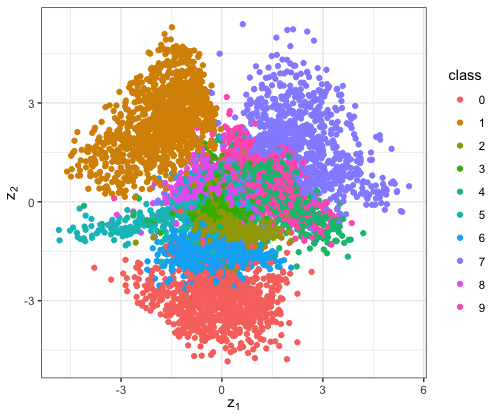
\includegraphics[width=0.9\textwidth]{fig/MNIST_VAE_latent.png}
\caption{The latent state of MNIST using an Variational Autoencoder}
\end{figure}

\end{frame}


%%%%%%%%%%%%%%%%%%%%%%%%%%%%%%%%%%%%%%%%%%%%%%%%%%%%%%%%%%%%%%%%%%

\section{Autoencoders}

\begin{frame}{Autoencoder}

\begin{itemize}
\item An autoencoder is a neural network (e.g. feed-forward) that take an input $x$ and predict (the same) $x$ ($r$). \pause
\item Three parts:
\begin{itemize}
\item {\color{uured}encoder} $f(x)$ (or $e(x)$)
\item code
\item {\color{uured}decoder} $g(h)$ (or $d(z)$)
\end{itemize}

\begin{figure}[h]
\centering
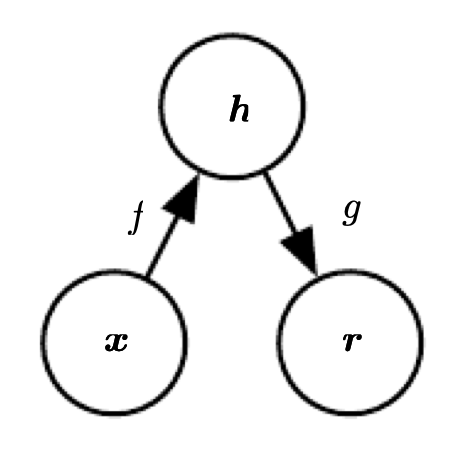
\includegraphics[width=0.3\textwidth]{fig/DL_14_1_ae}
\caption{A Neural Autoencoder (Goodfellow et al, 2018)}
\end{figure}

\pause

\item Loss function ({\color{uured}reconstruction error}):
\[
L(\phi, \theta) = (x - d_\phi(e_\theta(x)))^2
\]
\end{itemize}

\end{frame}



\begin{frame}{The Undercomplete Autoencoder}

\begin{itemize}
\item More interesting: an {\color{uured}undercomplete} autoencoder:\\Dimension of code is {\color{uured}lower} than that of $x$
\end{itemize}

\begin{figure}[h]
\centering
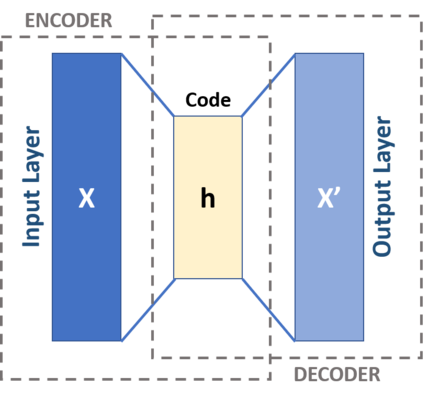
\includegraphics[width=0.6\textwidth]{fig/440px-Autoencoder_schema.png}
\caption{A Neural Autoencoder (Wikipedia)}
\end{figure}

\end{frame}


\begin{frame}{PCA and autoencoders}

\begin{itemize}
\item A linear autoencoder: $e_\theta(x) = W_\phi$, and $d_\theta(x) = W_\phi$
\item We want to minimize the loss (ignoring $b$/the mean):
\[
L(\phi, \theta) = \sum_{i=1}^N (x_i - W_\theta W_\phi x_i)^2
\]
\pause
\item Remember {\color{uured} PCA loss}:
\[
L(P) = \sum_{i=1}^N (x_i - P_q P_q^T x_i)^2\,,
\]
where $P$ is an orthogonal matrix of rank $q$.
\pause
\item {\color{uured} Hence}: PCA can be seen as an autoencoder
\end{itemize}

\begin{figure}[h]
\centering
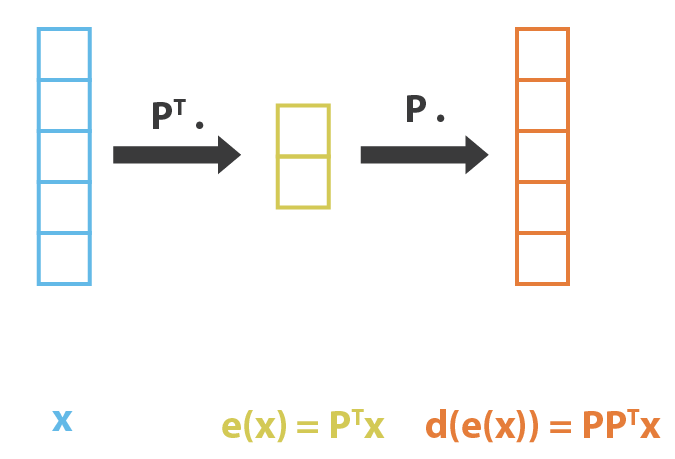
\includegraphics[width=0.6\textwidth]{fig/Rocca_PCA_as_autoencoder2.png}
\caption{PCA as autoencoder (Rocca, 2019)}
\end{figure}

\end{frame}


\begin{frame}{Deep Autoencoders}
\begin{itemize}
\item Deep Autoencoder: An autoencoder with {\color{uured} multilayer neural networks} as encoder and decoder
\begin{itemize}
\item can be seen as a non-linear PCA
\item learn nonlinear representations
%\item project data onto a nonlinear manifold
%(manifold is a topological space that locally resembles Euclidean space near each point)
\end{itemize}
\pause
\item Problem: Deep autoencoders needs to be {\color{uured} regularized} to not {\color{uured} overfit} the latent state
\end{itemize}

\end{frame}


\begin{frame}{probabilistic PCA as an decoder}

\begin{itemize}
\item Problem: Autoencoders (as PCA) are not probabilistic models:
\begin{itemize}
\item cannot generate data.
\item no notion of uncertainty
\end{itemize}
\item We would like something like probabilistic PCA for (deep) autoencoders\pause
\item Remember the pPCA model (with z as latent variable):
\[
x_i \sim N({\color{uured}b +  W} z_i^T, \sigma I)
\]
\pause
\item Now, swap the simple parameters with a neural network
\[
x_i \sim N({\color{uured}\text{NeuralNetwork}}_\phi (z_i), \sigma I)
\]
\pause
\item This is an example of a {\color{uured} Deep Latent Variable model}\\(a probabilistic decoder)
\item Another example is the {\color{uured} Variational Autoencoder}
\end{itemize}

\end{frame}

%%%%%%%%%%%%%%%%%%%%%%%%%%%%%%%%%%%%%%%%%%%%%%%%%%%%%%%%%%%%%%%%%%
\section{The Variational Autoencoder}

\begin{frame}{The Variational Autoencoder}
\begin{itemize}
\item The variational autoencoder (VAE) is a {\color{uured} deep probabilistic autoencoder}
\item Commonly used for unsupervised learning of {\color{uured} images}\pause
\item Consists of {\color{uured} three parts}:
\begin{enumerate}
\item The (probabilistic) encoder $q(z|\phi, x)$: inference model
\item Sample $z$ from encoded $x$
\item The (probabilistic) decoder $p(x|\theta, z)$: observation model
\end{enumerate}
\pause
\item Encoding the {\color{uured} latent state as a distribution} forces the space to be "reasonable"/reduces overfitting
\pause
\item VAEs get their name from {\color{uured} variational inference} (used in training)
\end{itemize}

\end{frame}


\begin{frame}{The Variational Autoencoder}

\begin{figure}[h]
\centering
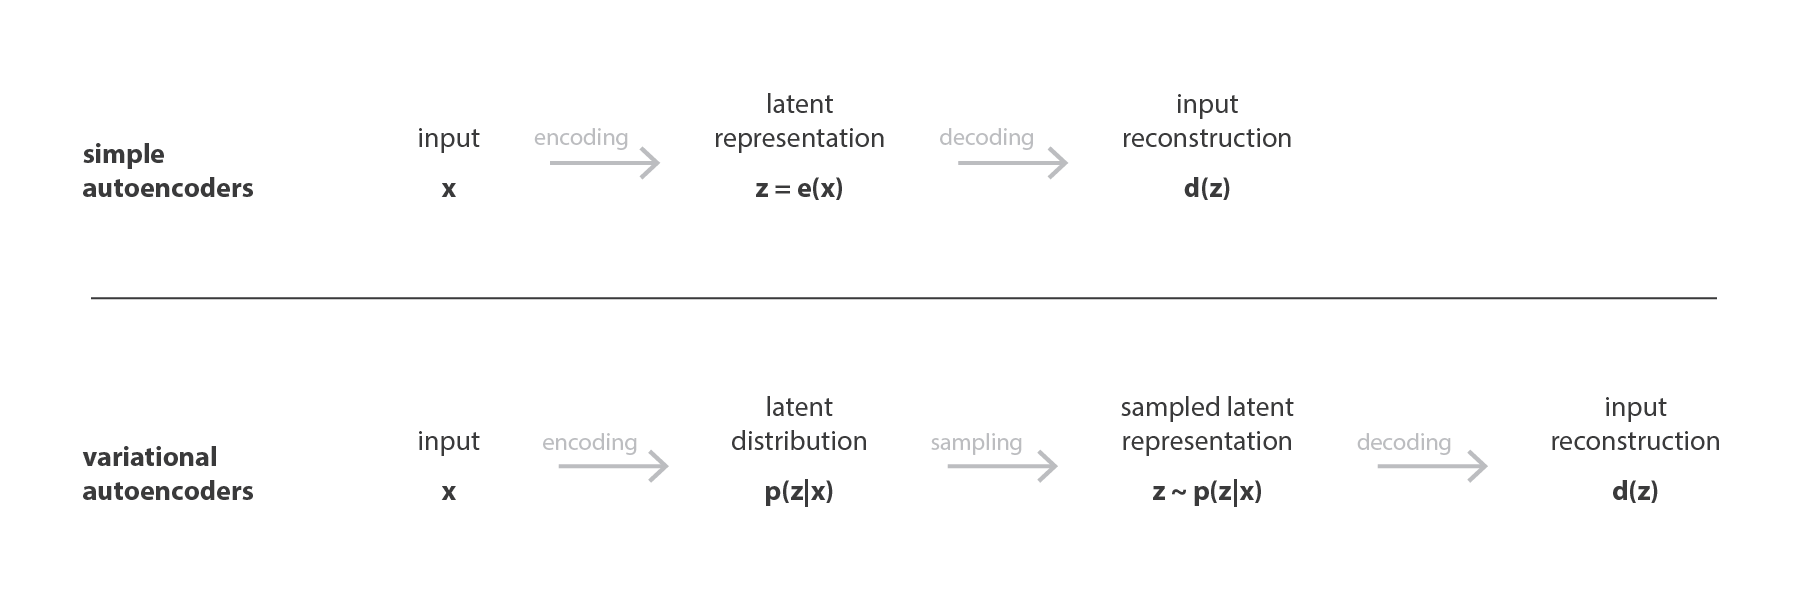
\includegraphics[width=1\textwidth]{fig/Rocca_AE_vs_VAE.png}
\caption{Autoencoder vs. the Variational Autoencoder (Rocca, 2019)}
\end{figure}

\end{frame}


\begin{frame}{The Variational Autoencoder}

\begin{figure}[h]
\centering
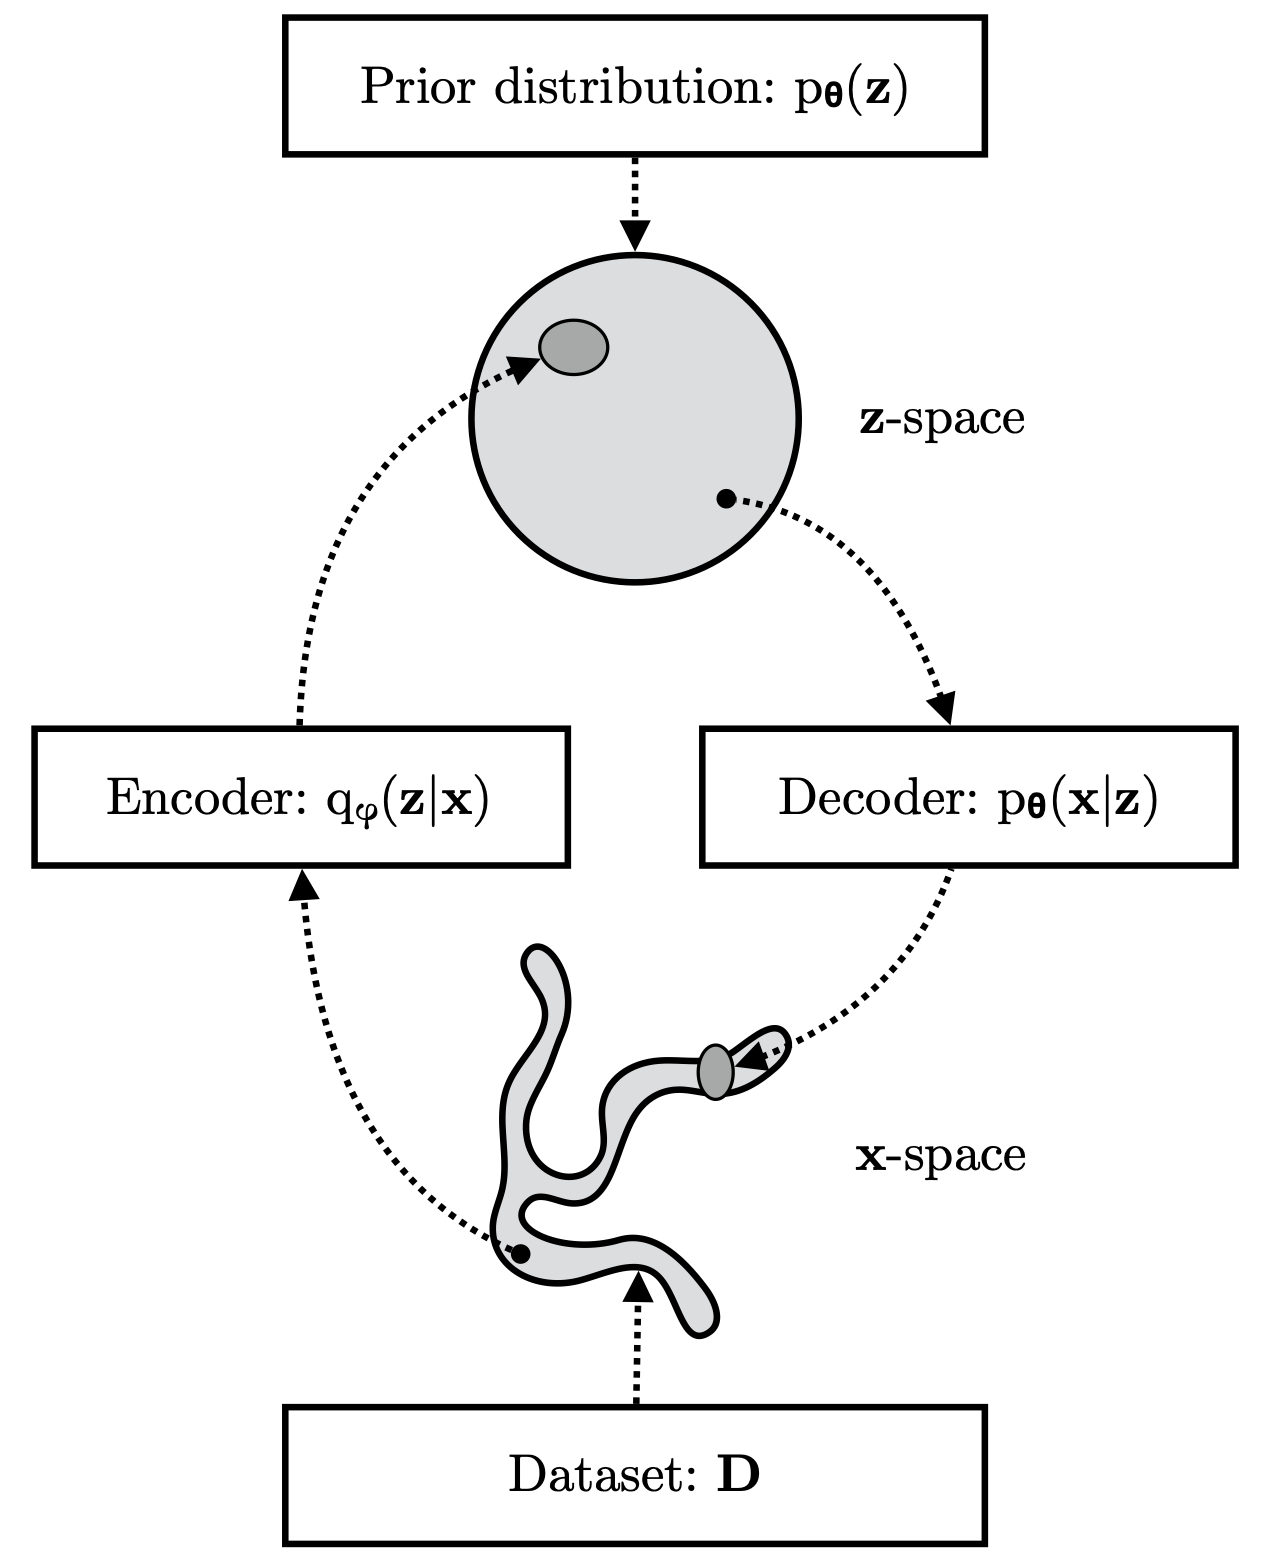
\includegraphics[width=0.6\textwidth]{fig/Kingma_Welling_2018_Fig_2_1.png}
\caption{The Variational Autoencoder (Kingma and Welling, 2018, Fig. 2.1)}
\end{figure}

\end{frame}


\subsection{The probabilistic decoder}

\begin{frame}{The probabilistic decoder}
\begin{itemize}
\item The probabilistic decoder $p(x|\theta, z)$ ({\color{uured} observation model})
\item Usually a Normal distribution:
\[
x_i \sim N(\text{NeuralNetwork}(z,\theta), c I)
\]
\item $x_i$ for observation $i$ depends non-linearly on $z_i$
\item A probabilistic linear decoder: {\color{uured} pPCA}
\end{itemize}

\begin{figure}[h]
\centering
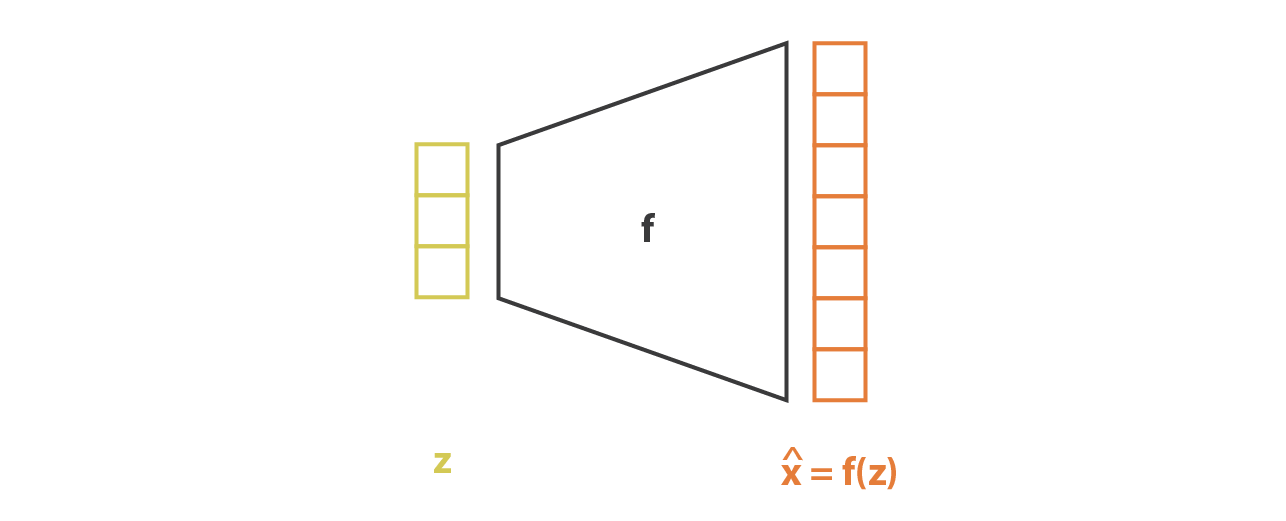
\includegraphics[width=0.8\textwidth]{fig/Rocca_VAE_decoder.png}
\caption{The Decoder (Rocca, 2019)}
\end{figure}

\end{frame}


\subsection{The probabilistic encoder}

\begin{frame}{The probabilistic encoder}

\begin{itemize}
\item The probabilistic encoder $q(z|x, \phi)$ ({\color{uured} inference model})
\item We want: $q_\phi(z|x) \approx p_\theta(z|x)$
\pause
\item We assume that $q_\phi(z|x)$ follows a specific distribution. Commonly:
\[
z \sim N(\mu, \Sigma)
\]
\item A neural network learns the parameters $\mu$ and $\Sigma$
\[
\mu = \text{NeuralNetwork}(x,\phi_\mu)\,, \Sigma = \text{NeuralNetwork}(x,\phi_\Sigma)\,,
\]
where $\phi = (\phi_\mu, \phi_\Sigma)$
\pause
\item One common assumption is that $\Sigma$ is a diagonal matrix.
\item {\color{uured} Result}: $z_i$ for observation $i$ depends non-linearly on $x_i$
\end{itemize}

\end{frame}

\begin{frame}{The probabilistic encoder}

\begin{figure}[h]
\centering
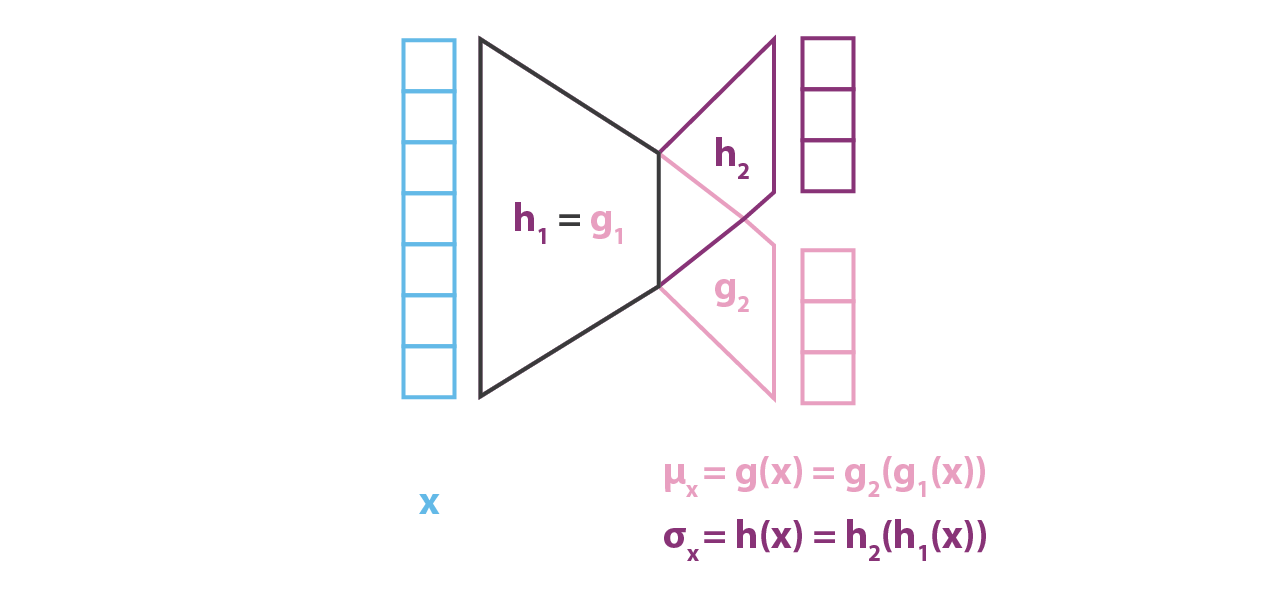
\includegraphics[width=1\textwidth]{fig/Rocca_VAE_encoder.png}
\caption{The Encoder (Rocca, 2019)}
\end{figure}

\end{frame}



\begin{frame}{The Variational Autoencoder}

\begin{figure}[h]
\centering
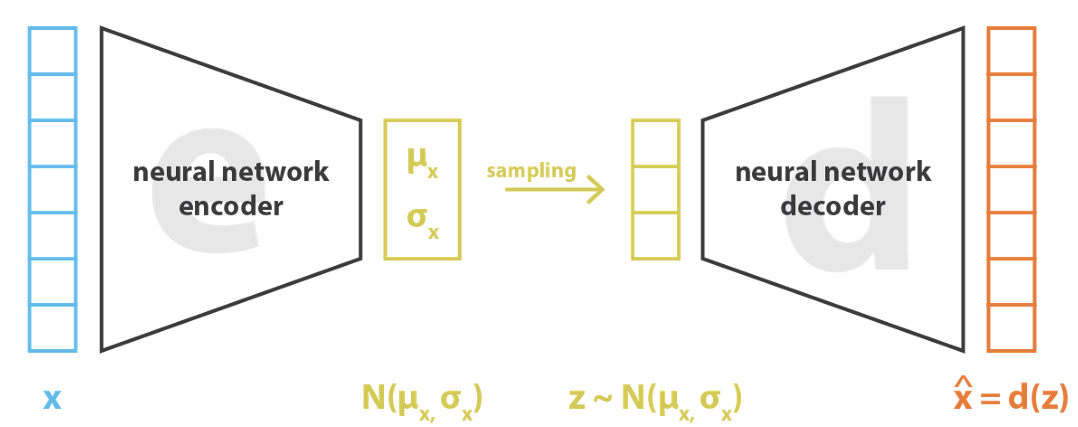
\includegraphics[width=0.8\textwidth]{fig/Rocca_VAE2.png}
\caption{The Variational Autoencoder (Rocca, 2019)}
\end{figure}

\end{frame}


\begin{frame}{The Variational Autoencoder}

\begin{figure}[h]
\centering
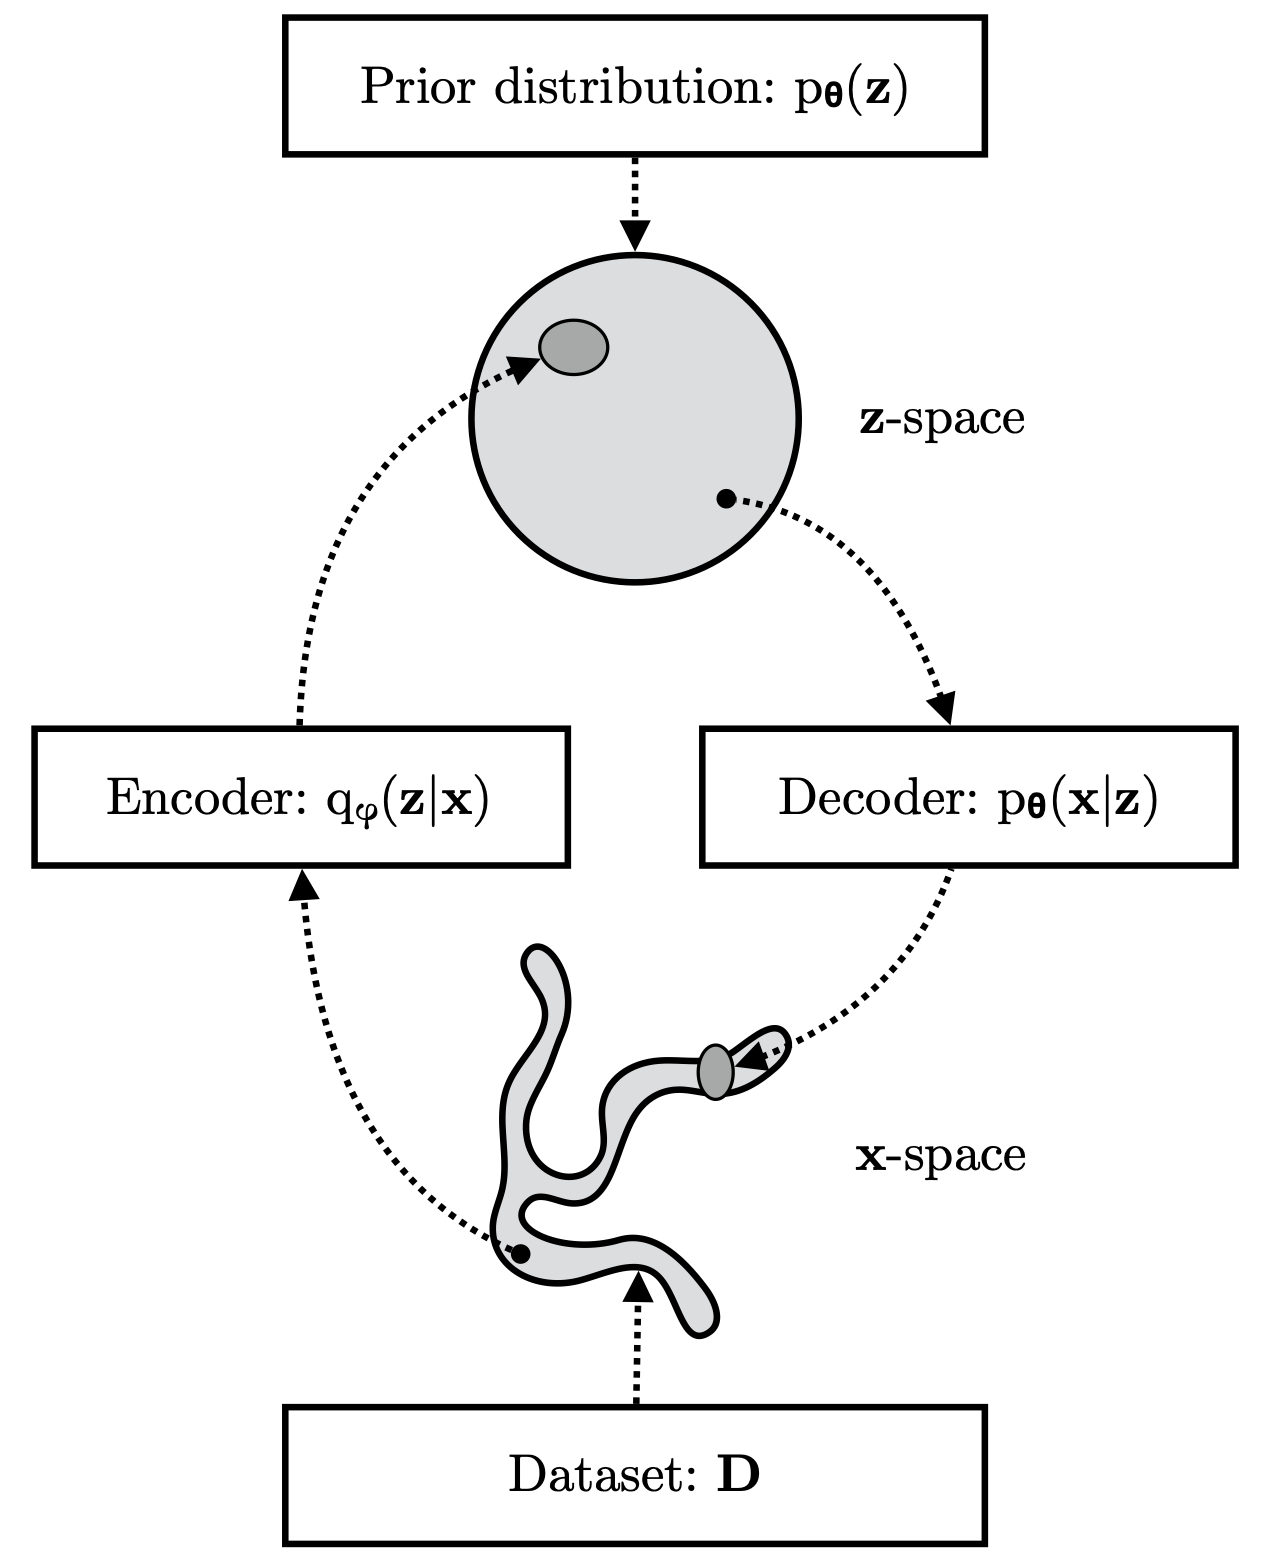
\includegraphics[width=0.6\textwidth]{fig/Kingma_Welling_2018_Fig_2_1.png}
\caption{The Variational Autoencoder (Kingma and Welling, 2018, Fig. 2.1)}
\end{figure}
\end{frame}

\subsection{Traing a variational autoencoder}

\begin{frame}{Training a VAE}
\begin{itemize}
\item {\color{uured} Goal}: estimating $\phi$, $\theta$ (and $z_i$)
%\item We have a sampling step in the middle (the latent state $z$)
\item The encoder and decoder are (usually) complicated \\ (no close form solution)
\item Need to estimate $\phi$ and $\theta$ using gradient ascent
\item Target:
\begin{itemize}
\item Maximize $\log p(x)$\\(Explain the data as well as possible)
\end{itemize}\pause
\item Optimization target: \\Maximize the variational lower bound or {\color{uured} evidence lower bound (ELBO)}
\end{itemize}
\end{frame}


\begin{frame}{The marginal log-likelihood}

\begin{align*}
\log p_\theta(x)&={\color{uured}\int q_\phi(z|x)} \log p_\theta(x) {\color{uured} dz}&  \\
&={\color{uured}\mathbb{E}_{q_\phi(z|x)}}[\log p_\theta(x)] \\
&=\mathbb{E}_{q_\phi(z|x)}\left[\log \left({\color{uured}\frac{p_\theta(x,z)}{p_\theta(z|x)}}\right)\right]\,, \text{using}\, p(z|x)= \frac{p(x,z)}{p(x)} \\
&=\mathbb{E}_{q_\phi(z|x)}\left[\log \left(\frac{p_\theta(x,z)}{{\color{uured}q_\phi(z|x)}}\frac{{\color{uured}q_\phi(z|x)}}{p_\theta(z|x)}\right)\right] \\
&=\mathbb{E}_{q_\phi(z|x)}\left[\log \left(\frac{p_\theta(x,z)}{q_\phi(z|x)}\right)\right] + \mathbb{E}_{q_\phi(z|x)}\left[\log \left(\frac{q_\phi(z|x)}{p_\theta(z|x)}\right)\right] \\
&=\underbrace{\mathcal{L}_{\theta,\phi}(x)}_{\text{ELBO}} + D_{KL}(q_\phi(z|x)||p_\theta(z|x))\\
\end{align*}
\pause
\begin{align*}
\underbrace{\mathcal{L}_{\theta,\phi}(x)}_{\text{ELBO}} = \log p_\theta(x) - D_{KL}(q_\phi(z|x)||p_\theta(z|x))
\end{align*}

\end{frame}


\begin{frame}{The Kullback-Leibler divergence}

\begin{itemize}
\item {\color{uured} The Kulback-Leibler divergence}: a way of measuring the distance between probability distributions (although, not a metric)
\[
D_{KL}(q_\phi(z|x)||p_\theta(z|x)) = \mathbb{E}_{q_\phi(z|x)}\left[\log \left(\frac{q_\phi(z|x)}{p_\theta(z|x)}\right)\right]
\]

\[
D_{KL}(q_\phi(z|x)||p_\theta(z|x)) \geq 0
\]
\end{itemize}

\end{frame}


\begin{frame}{Training target}

\begin{itemize}
\item Optimization target: Maximize the ELBO
\begin{align*}
\mathcal{L}_{\theta,\phi}(x) = \log p_\theta(x) - D_{KL}(q_\phi(z|x)||p_\theta(z|x))
\end{align*}
\item ELBO is a lower bound for the marginal log-likelihood\\ (similar to the EM algorithm)
\pause
\item Maximizing the ELBO will do two things:
\begin{itemize}
\item Maximize the marginal log-likelihood $\log p_\theta(x)$:\\Better generative model/decoder
\item Minimize the KL-divergence between $q_\phi(z|x)$ and $p_\theta(z|x)$:\\Better approximation of the latent space/encoder
\end{itemize}
\end{itemize}

\end{frame}



\begin{frame}{Optimizing the ELBO}

\begin{itemize}
\item Stochastic Gradient \emph{Ascent} to maximize:
\begin{align*}
\mathcal{L}_{\theta,\phi}(x) =& \sum_i^N \mathcal{L}_{\theta,\phi}(x_i)\\
=& \sum_i^N \mathbb{E}_{q_\phi(z_i|x_i)}\left[\log \left(p_\theta(x_i,z_i)\right) - \log(q_\phi(z_i|x_i))\right]
\end{align*}
\pause
\item Two problems:
\begin{enumerate}
\item How do we compute the expectation? \\ Solution: {\color{uured} Monte Carlo Approximation}\pause
\item How compute the gradient wrt $\phi$?\\ Solution: {\color{uured}Change of variables}: $z = g(\epsilon, \phi, x)$\\This is called {\color{uured}the reparametrization trick}
\end{enumerate}
\end{itemize}

\end{frame}

\begin{frame}{Optimizing the ELBO}

\begin{itemize}
\item Using the reparametrization trick and Monte Carlo approximation, we get:
\begin{align*}
\mathcal{L}_{\theta,\phi}(x) =& \mathbb{E}_{q_\phi(z|x)}\left[\log \left(p_\theta(x,z)\right)- \log(q_\phi(z|x))\right]\\
 =& \mathbb{E}_{p(\epsilon)}\left[\log \left(p_\theta(x,g(\epsilon, \phi, x))\right)- \log(q_\phi(g(\epsilon, \phi, x)|x))\right]\\
 \approx & \log \left(p_\theta(x,g(\epsilon, \phi, x))\right)- \log(q_\phi(g(\epsilon, \phi, x)|x))
\end{align*}
\pause
\item A common approach: do the MC approximation with only {\color{uured}one sample per datapoint $x_i$}.\pause
%\item unbiasedness
\item We approximate both $\mathcal{L}_{\theta,\phi}(x)$ and $\nabla\mathcal{L}_{\theta,\phi}(x)$
\pause
\item Sometimes called a {\color{uured}doubly stochastic} algorithm.
\end{itemize}

\end{frame}


\begin{frame}{The Autoencoding Variational Bayes Algorithm}

\begin{figure}[h]
\centering
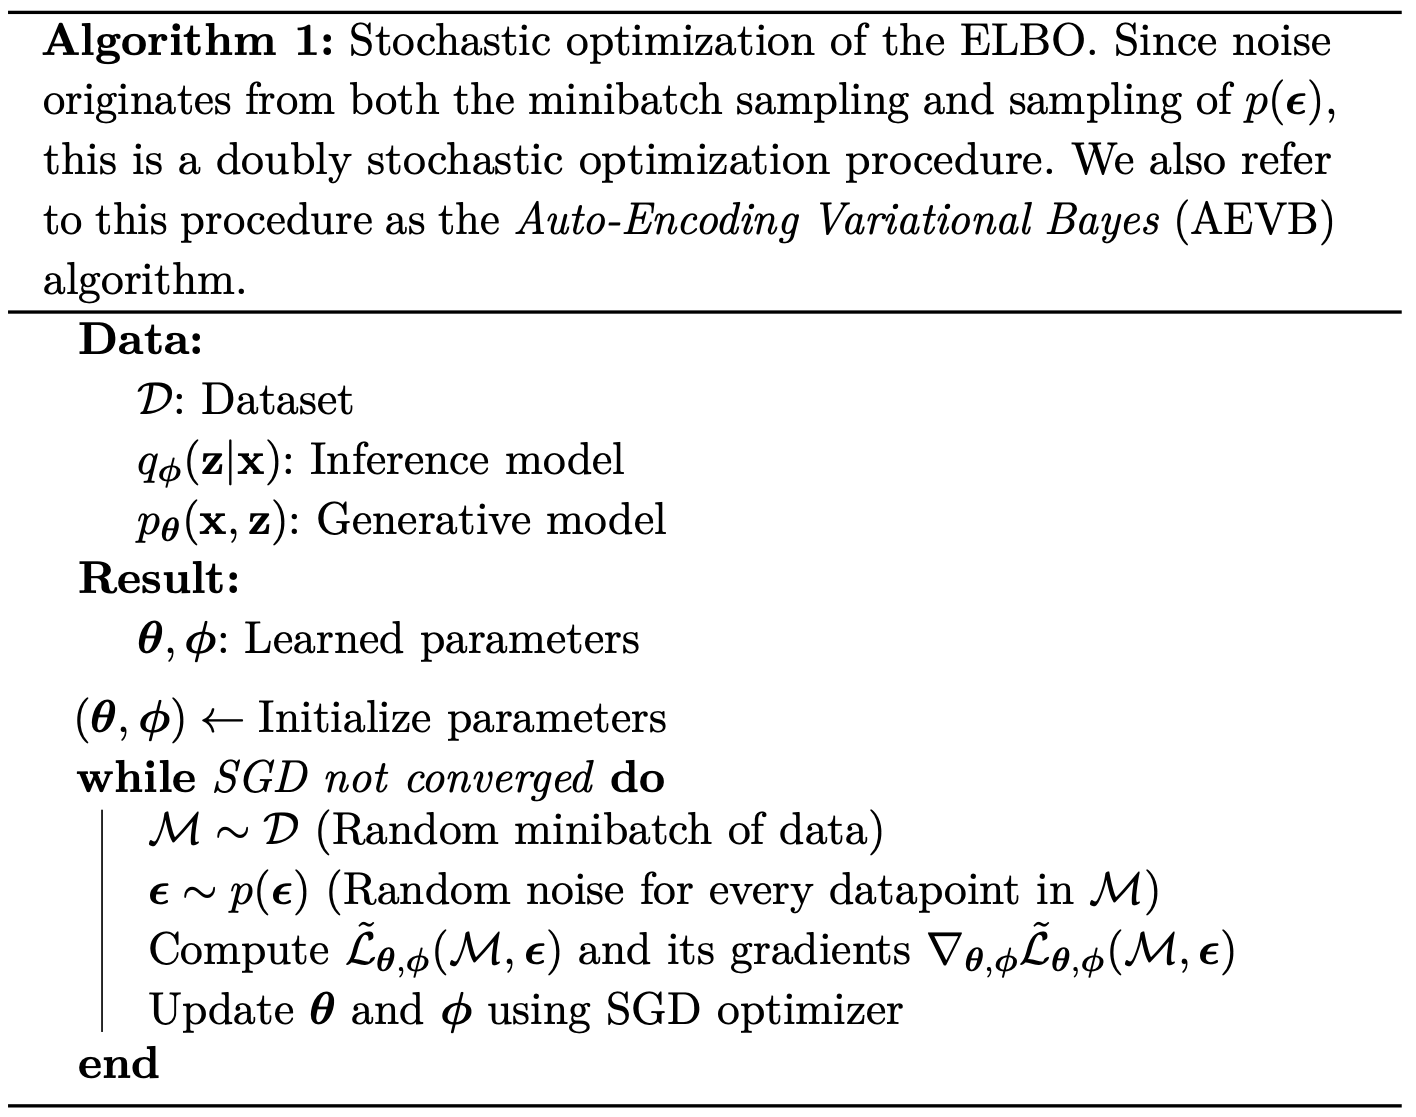
\includegraphics[width=0.8\textwidth]{fig/Kingma_Welling_2018_Algo_1.png}
\caption{The Autoencoding Variational Bayes Algorithm (Kingma and Welling, 2018, Algo. 1)}
\end{figure}

\end{frame}


\begin{frame}{The Autoencoding Variational Bayes Algorithm}

\begin{figure}[h]
\centering
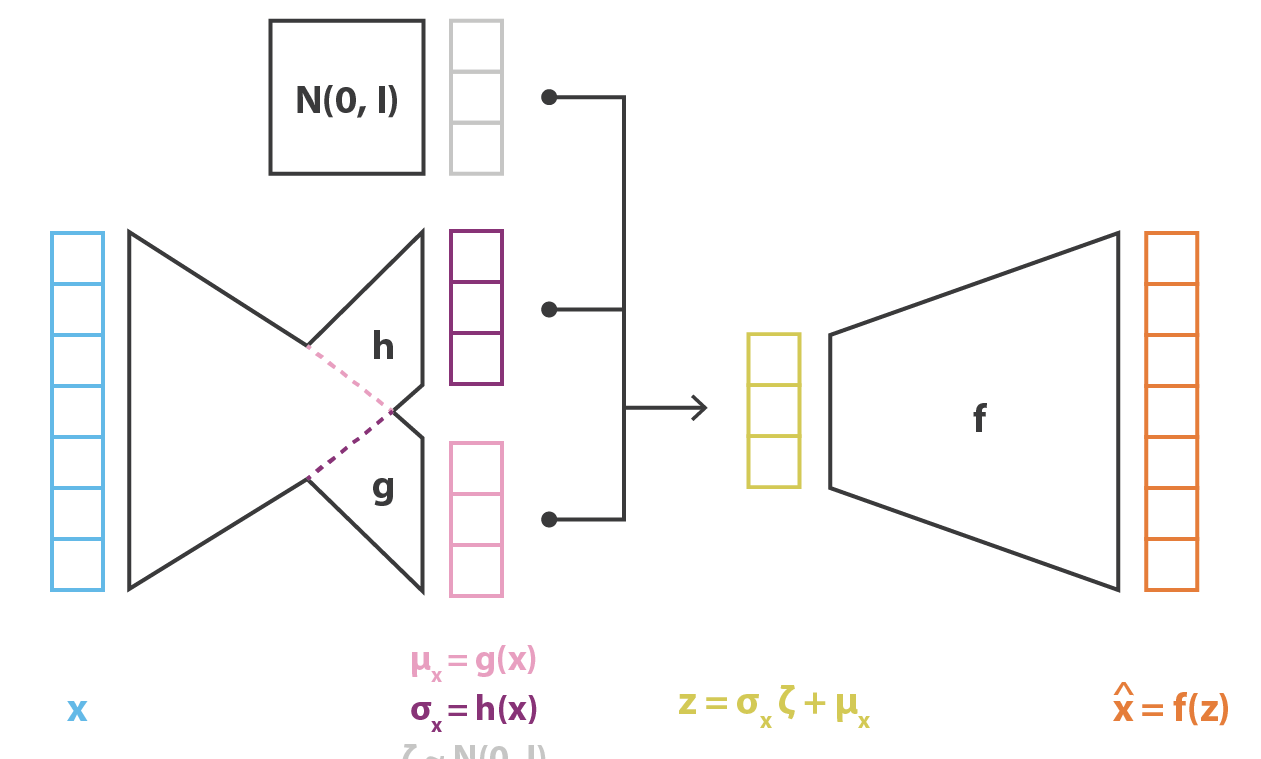
\includegraphics[width=0.8\textwidth]{fig/Rocca_VAE_full_reparmetr.png}
\caption{The Autoencoding Variational Bayes Algorithm (Rocca, 2019)}
\end{figure}

\end{frame}

\begin{frame}{Summary}

\begin{itemize}
\item Benefits of VAE:
\begin{itemize}
\item Get a more interpretable latent state
\item We can estimate uncertainty
\item We can inject knowledge in our latent state
\end{itemize}
\pause
\item Problems:
\begin{itemize}
\item The blurry image problem % Examples. probably due to the prior and latent state
\end{itemize}
\pause
\item Still much ongoing research:
\end{itemize}

\begin{figure}[h]
\centering
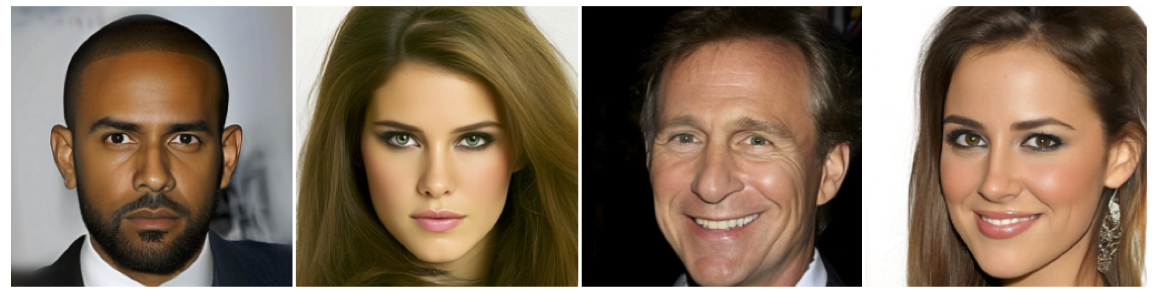
\includegraphics[width=0.8\textwidth]{fig/Vahdat_Kautz_NVEA_2020.png}
\caption{Examples of images generated with a deep hierarchical Variational Autoencoder (Vahdat and Kautz, 2020)}
\end{figure}

\end{frame}



%%%%%%%%%%%%%%%%%%%%%%%%%%%%%%%%%%%%%%%%%%%%%%%%%%%%%%%%%%%%%%%%%%%%%%%%%%%%%%%%
\section{Probabilistic Topic Models}

\frame{\sectionpage}

\begin{frame}{Probabilistic Topic Models}

\begin{itemize}
    \item Unsupervised method for {\color{uured} textual data}\pause
    \item Popular in industry and academia to {\color{uured} analyze large corpora}\pause
    \item The most common model: {\color{uured} Latent Dirichlet Allocation}
    \item A {\color{uured} mixed membership} model (a mixture of multinomial mixtures model)\pause
    \item Topic model builds on the the {\color{uured} distributional hypothesis}\pause
    \item Use cases:
    \begin{itemize}
        \item Create features for supervised models\pause
        \item Integrated in neural networks for model efficient learning\pause
        \item Visualize document collections\pause
        \item Analyzing large corpora using statistical methods\pause
    \end{itemize}
    \item Example: {\color{uured} All ears} media monitoring of speech data
\end{itemize}
\end{frame}



\begin{frame}{The Dirichlet Distribution}

\begin{itemize}
    \item Probability distribution over the simplex with $K$ categories:
\[
f({\boldsymbol {x} }| {\boldsymbol {\alpha }}) = {\frac {1}{\mathrm {B} ({\boldsymbol {\alpha }})}} \prod _{i=1}^{K}x_{i}^{\alpha _{i}-1}\,
\]
where
\[
{\displaystyle \mathrm {B} ({\boldsymbol {\alpha }})={\frac {\prod _{i=1}^{K}\Gamma (\alpha _{i})}{\Gamma {\bigl (}\sum _{i=1}^{K}\alpha _{i}{\bigr )}}}}\,,
\]
and where
\[
{\displaystyle {\boldsymbol {\alpha }}=(\alpha _{1},\ldots ,\alpha _{K})}
\]\pause
\item The probability distribution has the support on the simplex, that is
\[
    \sum_{i=1}^{K}x_{i}=1{\text{ and }}x_{i}\geq 0{\text{ for all }} i\in [1,K]
\]
\pause
\item The parameters ${\boldsymbol {\alpha }}$ can be seen as {\color{uured} pseudo-counts}
\end{itemize}
\end{frame}


\begin{frame}{The Dirichlet Distribution}


\begin{figure}[h]
\centering
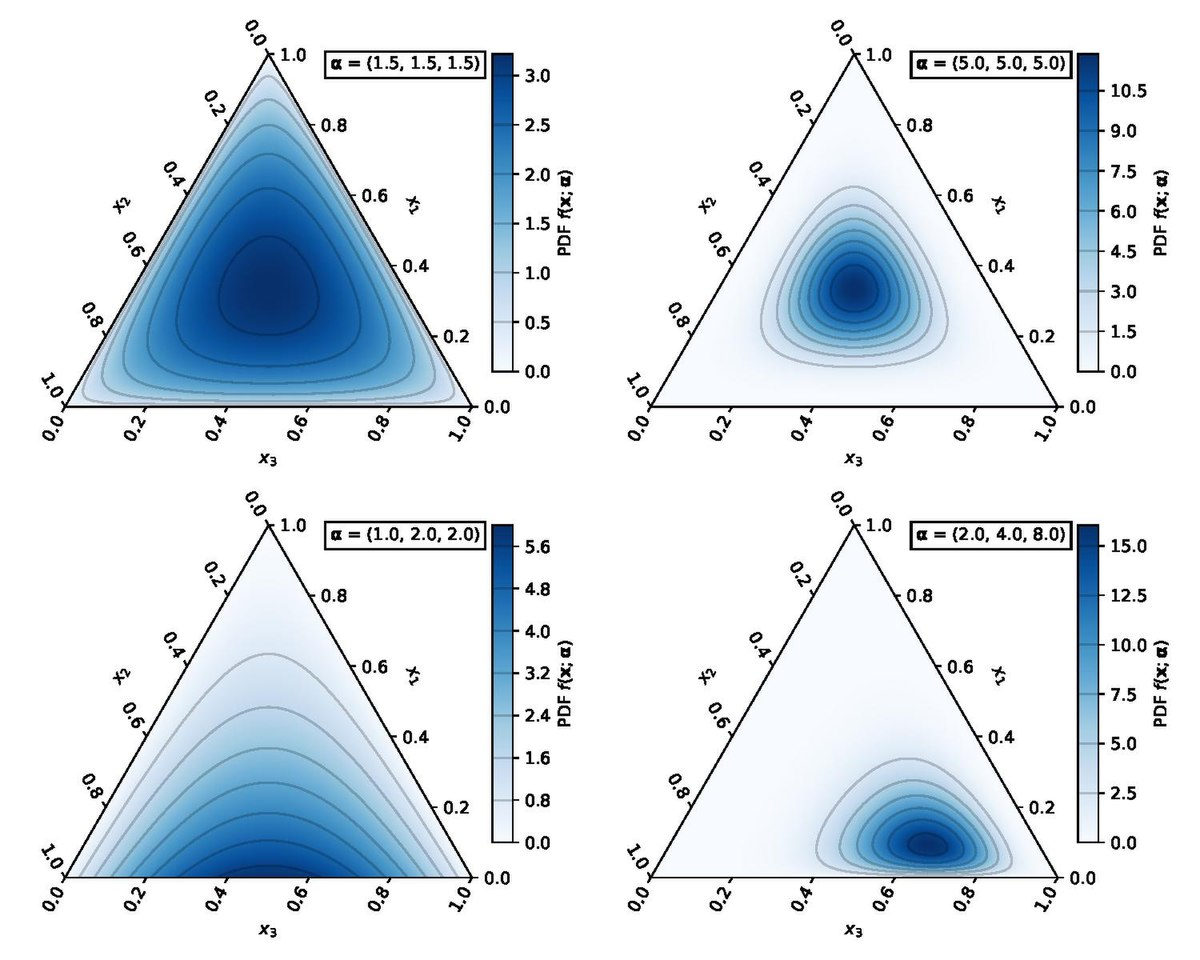
\includegraphics[width=0.8\textwidth]{fig/dirichlet.jpg}
\caption{The Dirichlet Distribution (Wikipedia)}
\end{figure}

\end{frame}



\begin{frame}{The distributional hypothesis}

\begin{itemize}
    \item Harris (1954) and Firths (1957): \\ ``Word is characterized by the company it keeps''
    \pause
    \item Semantics (broadly defined) is captured by {\color{uured} context}\pause
    \item Rough definition: {\color{uured} word windows} of different sizes\pause
    \item Different window sizes, different {\color{uured} semantic} content:
    \begin{itemize}
      \item Word embeddings (context: word windows)
      \item Topic models (context: documents)
    \end{itemize}
\end{itemize}

\begin{example}
\begin{enumerate}
    \item ``A friend in need is a friend indeed.''
    \item ``She is my friend indeed.''
\end{enumerate}
\end{example}
\end{frame}




%%%%%%%%%%%%%%%%%%%%%%%%%%%%%%%%%%%%%%%%%%%%%%%%%%%%%%%%%%%%%%%%%%%%%%%%%%%%%%%%
\subsection{Latent Dirichlet Allocation}

\begin{frame}{Latent Dirichlet Allocation}

\begin{figure}[h]
\centering
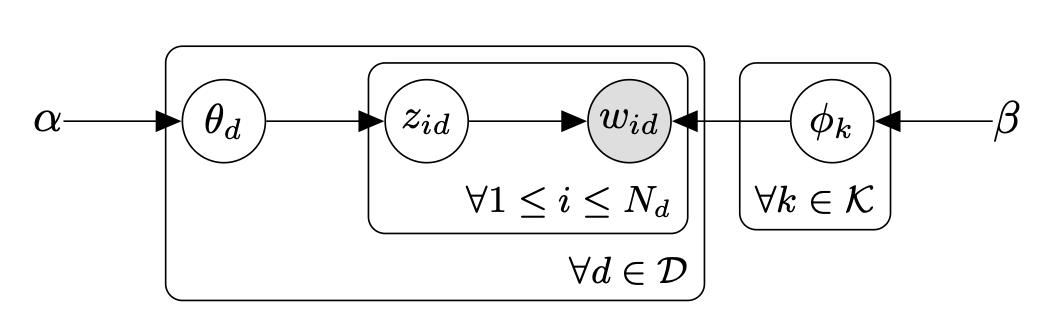
\includegraphics[width=0.8\textwidth]{fig/lda_model.png}
\caption{The Latent Dirichlet Allocation Model}
\end{figure}
where $\phi_k$ is the $k$th row in $\Phi$ (of dimension $K \times V$) and $\theta_d$ is the $d$th row in $\Theta$ (of dimension $D \times K$).

\end{frame}

\begin{frame}
\frametitle{Generative model for LDA}


Relies on the {\color{uured} bag-of-word} assumption
% Not much better with BERT embeddings


\begin{enumerate}
    \item For each component $k$ to $K$:
    \begin{enumerate}
        \item $\phi_k \sim$ Dirichlet($\beta$)
    \end{enumerate}
    \item For each document $d$:
    \begin{enumerate}
        \item $\theta_d \sim$ Dirichlet($\alpha$)
        \item For each token $i$:
        \begin{enumerate}
            \item $z_{id} \sim$  Categorical($\theta_d$)
            \item $w_{id} \sim$  Categorical($\phi_{z_{id}}$)
        \end{enumerate}
    \end{enumerate}
\end{enumerate}

\end{frame}


\begin{frame}{Example of parameters  $\mathbf{z}$, $\Theta$ and $\Phi$}

\[
\begin{array}{ccccccc}
\mathbf{w}_{1} &  & \mbox{boat} & \mbox{shore} & \mbox{bank}\\
\mathbf{z}_{1} &  & 1 & 1 & 1\\
\mathbf{w}_{2} &  & \mbox{Zlatan} & \mbox{boat} & \mbox{shore} & \mbox{money} & \mbox{bank}\\
\mathbf{z}_{2} &  & 2 & 1 & 1 & 3 & 3\\
\mathbf{w}_{3} &  & \mbox{money} & \mbox{bank} & \mbox{soccer} & \mbox{money}\\
\mathbf{z}_{3} &  & 3 & 3 & 2 & 3
\end{array}
\]
\pause
\[
\Phi=\begin{array}{ccccccc}
 & \mbox{boat} & \mbox{shore} & \mbox{soccer} & \mbox{Zlatan} & \mbox{bank} & \mbox{money}\\
\text{Topic 1} & 0.35 & 0.35 & 0.05 & 0.05 & 0.15 & 0.05\\
\text{Topic 2} & 0.025 & 0.025 & 0.45 & 0.45 & 0.025 & 0.025\\
\text{Topic 3} & 0.025 & 0.025 & 0.025 & 0.025 & 0.45 & 0.45
\end{array}
\]
\pause
\[
\Theta=\begin{array}{cccc}
 & \text{Topic 1} & \text{Topic 2} & \text{Topic 3}\\
\text{doc 1} & 0.96 & 0.02 & 0.02\\
\text{doc 2} & 0.3 & 0.2 & 0.5\\
\text{doc 3} & 0.05 & 0.35 & 0.6
\end{array}
\]


\end{frame}




%%%%%%%%%%%%%%%%%%%%%%%%%%%%%%%%%%%%%%%%%%%%%%%%%%%%%%%%%%%%%%%%%%%%%%%%%%%%%%%%
%%%% EXAMPLE OF LDA


\begin{frame}
\frametitle{}

\begin{displayquote}
Closing arguments were heard yesterday in the Federal bankruptcy fraud trial of Stephen J. Sabbeth, whose legal problems have raised doubts about his ability to continue as leader of the Nassau County Democratic Party.

\medskip

Mr. Sabbeth is charged with trying to conceal \$750,000 from his bank creditors by hiding the money in a secret account in his wife's maiden name, rather than use it to pay creditors when his lumber business went into bankruptcy 10 years ago.

\end{displayquote}

\hspace{10mm} -- The New York Times 25th of Febuary 1999

\end{frame}

\begin{frame}
\frametitle{The estimated topic proportion $(\hat{\theta_d})$}

\begin{center}
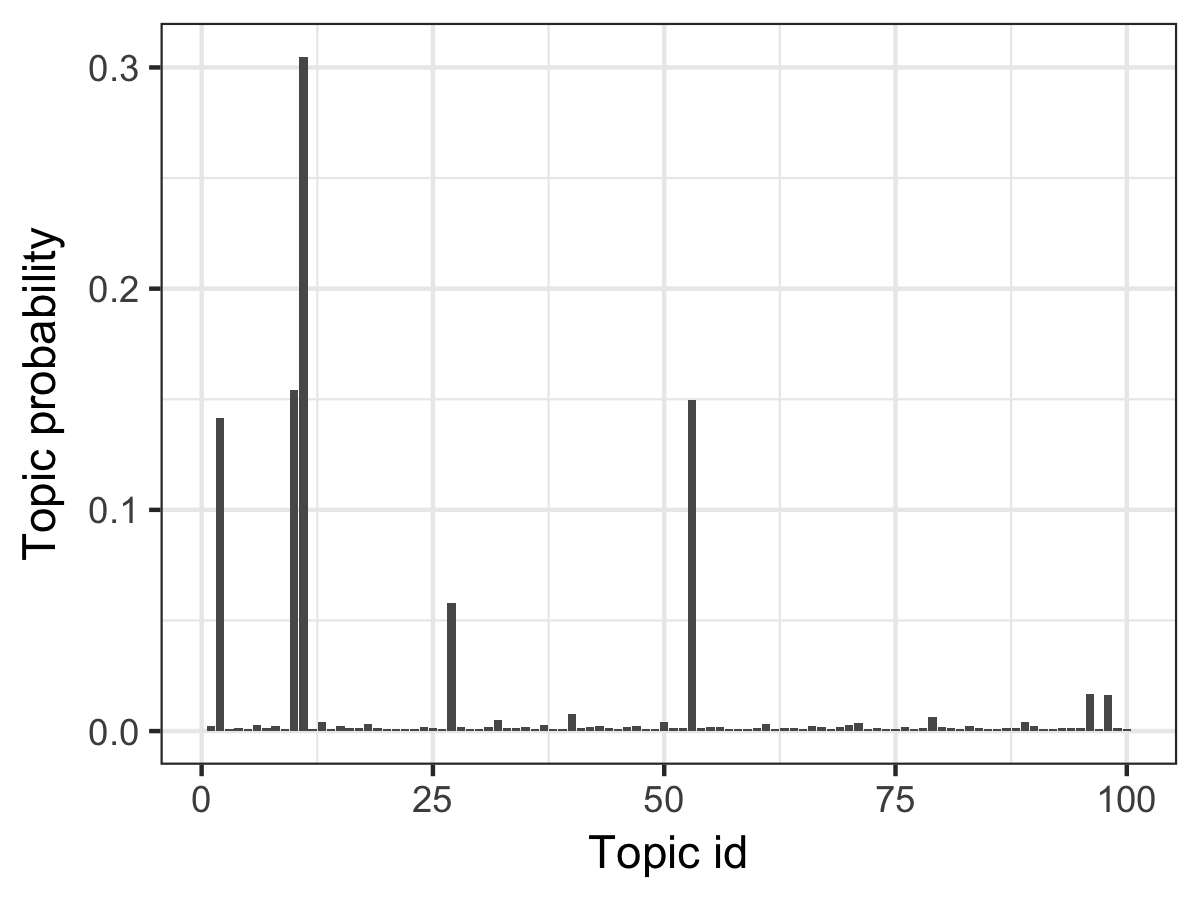
\includegraphics[width=0.7\textwidth]{fig/topic_prop.png}
\end{center}

\end{frame}

\begin{frame}
\frametitle{Topic top words}

\begin{table}[ht]
\centering
\begin{tabular}{llr}  
\toprule
%\multicolumn{2}{c}{Item} \\
%\cmidrule(r){1-2}
Topic    & Top words (by $\phi_{kv}$) \\
\midrule
  2 & party election voters campaign democratic \\
 10 & bank banks loans loan insurance savings \\
 11 & trial prison jury prosecutors convicted guilty \\
 53 & investigation inquiry documents investigators \\
%  2 & party election voters campaign democratic vote candidates \\
% 10 & bank banks loans loan insurance savings banking credit \\
% 11 & trial prison jury prosecutors convicted guilty charges case \\
% 53 & investigation inquiry documents investigators officials report \\ 
\bottomrule
\end{tabular}
\caption{The words with highest probability ($p(w|k)$) for topic 2, 10, 11 and 53.}
\label{example_top_words}
\end{table}

\end{frame}

\begin{frame}
\frametitle{The Latent Dirichlet Allocation Model}

\begin{figure}[h]
\begin{center}
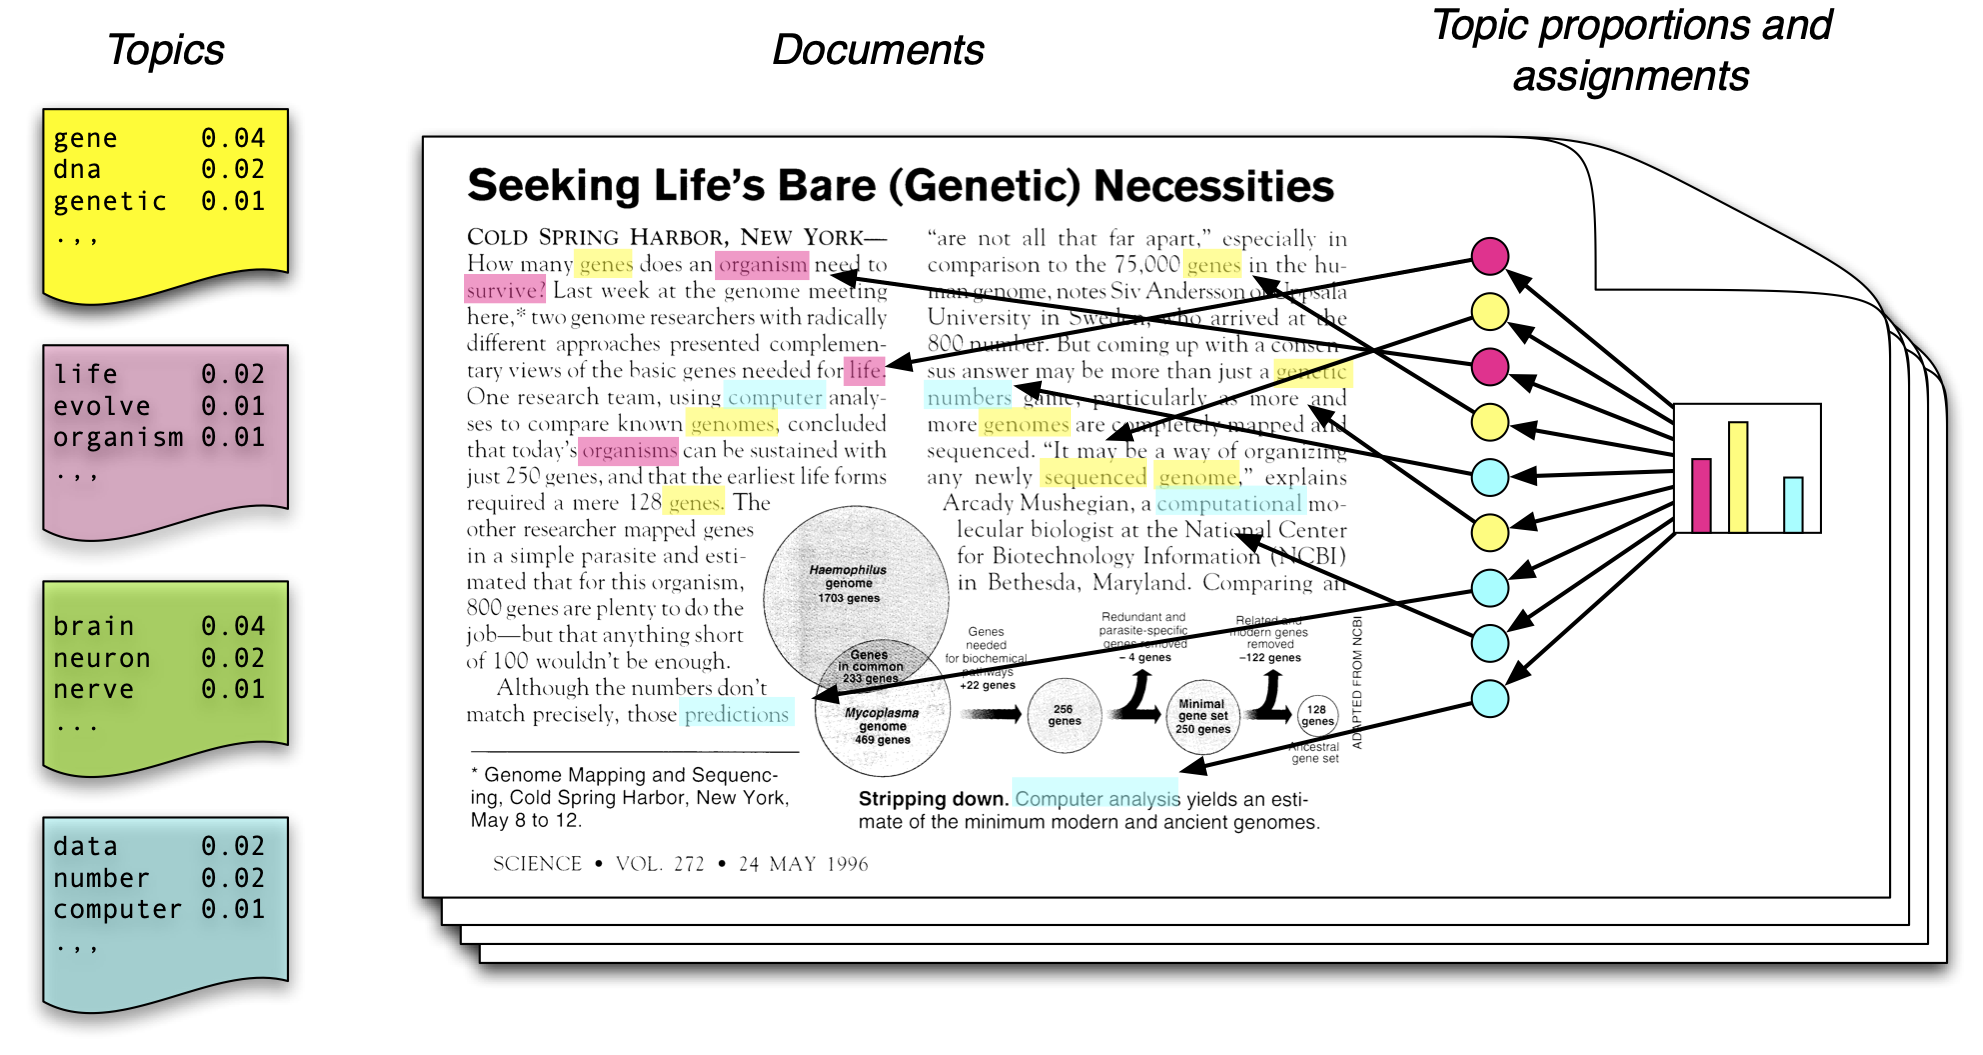
\includegraphics[width=0.9\textwidth]{fig/Blei2012_fig_1.png}
\caption{The Latent Dirichlet Allocation Model (Blei 2012, Fig. 1)}
\end{center}
\end{figure}

\end{frame}


%%%%%%%%%%%%%%%%%%%%%%%%%%%%%%%%%%%%%%%%%%%%%%%%%%%%%%%%%%%%%%%%%%%%%%%%%%%%%%%%
\subsection{Estimating the LDA model}

\begin{frame}
\frametitle{Inference}

\begin{itemize}
\item Common inference approaches

\begin{enumerate}
\item Variational inference %\cite{blei2003latent}
\item Markov Chain Monte Carlo (MCMC) %\cite{griffiths2004finding}
\end{enumerate}
\pause
\item The Gibbs sampler is usually prefered
\item Similar to (Stochastic) EM
\end{itemize}

\end{frame}



\begin{frame}{Gibbs sampler for LDA}

The basic Gibbs sampler:
\begin{enumerate}
\item We want to estimate $z, \Phi, \Theta$:
\pause
\item Sample topic indicators (latent variable)
\[
p(z=k|\Phi,\Theta)\propto\phi_{v,k}\theta_{k,d}
\]
\pause
\item Sample model parameters
\[
\theta_{d}|\mathbf{z}\sim Dir(\mathbf{n}^{(d)}+\alpha)
\]
\[
\phi_{k}|\mathbf{z}\sim Dir(\mathbf{n}^{(v)}+\beta)
\]
\end{enumerate}

where $\mathbf{n}^{(d)}$ is the number of tokens by topic in document
$d$ and $\mathbf{n}^{(v)}$ is the number of tokens by topic for word
type $v$.
\end{frame}

\begin{frame}{Gibbs sampler for LDA}

Integrating out (collapsing) $\Theta$ and $\Phi$ %(\citet{Griffiths2004}):
\begin{eqnarray*}
p(\mathbf{z}|\mathbf{w}) & = & \int\int p(\mathbf{z},\Theta,\Phi|\mathbf{w})\cdot p(\mathbf{z},\Theta,\Phi)d\mbox{\ensuremath{\Phi}}d\mbox{\ensuremath{\Theta}}
\end{eqnarray*}
will result in the following Gibbs sampler:

\[
p(z_{i}=k|w_{i},\mathbf{z}_{\lnot i})\propto\underbrace{\frac{n_{k}^{(v)}+\beta}{n_{k}^{(v)}+V\beta}}_{type-topic\mbox{ }\mbox{(\ensuremath{\Phi})}}\cdot\underbrace{(n_{k}^{(d)}+\alpha)}_{topic-doc\mbox{ }\mbox{(\ensuremath{\Theta})}}
\]
where $n^{(v)}$ and $n^{(d)}$ are count matrices of size $D\times K$
and $K\times V$.
\end{frame}


\begin{frame}{Example of $n^{(v)}$ and $n^{(d)}$}

\[
\begin{array}{ccccccc}
\mathbf{w}_{1} &  & \mbox{boat} & \mbox{shore} & \mbox{bank}\\
\mathbf{z}_{1} &  & 1 & 1 & 1\\
\mathbf{w}_{2} &  & \mbox{Zlatan} & \mbox{boat} & \mbox{shore} & \mbox{money} & \mbox{bank}\\
\mathbf{z}_{2} &  & 2 & 1 & 1 & 3 & 3\\
\mathbf{w}_{3} &  & \mbox{money} & \mbox{bank} & \mbox{soccer} & \mbox{money}\\
\mathbf{z}_{3} &  & 3 & 3 & 2 & 3
\end{array}
\]


\pause{}

\[
n^{(v)}=\begin{array}{cccccc}
\mbox{boat} & \mbox{shore} & \mbox{soccer} & \mbox{Zlatan} & \mbox{bank} & \mbox{money}\\
2 & 2 & 0 & 0 & 1 & 0\\
0 & 0 & 1 & 1 & 0 & 0\\
0 & 0 & 0 & 0 & 2 & 2
\end{array}
\]


\pause{}

\[
n^{(d)}=\left[\begin{array}{ccc}
3 & 0 & 0\\
2 & 1 & 3\\
0 & 2 & 3
\end{array}\right]
\]

\end{frame}



\begin{frame}{Topic Models as non-negative matrix factorization}
%\Small
%\begin{figure}
\begin{centering}
\[
\begin{array}{ccccc}
\\
\left[\begin{array}{ccc}
 & \text{ }\\
\\
\text{ } & n_{dv} & \text{ }\\
 & (D\times V)\text{ }\\
\\
\end{array}\right] & \approx & \left[\begin{array}{c}
\\
\\
\Theta\\
(D\times K)\\
\\
\end{array}\right] & \times & \left[\begin{array}{ccccc}
 &  & \text{ }\\
\text{ } & \text{ } & \Phi & \text{ } & \text{ }\\
 &  & (K\times V)
\end{array}\right]\\
\\
\end{array}
\]
\end{centering}
%\caption{Conceptual depiction of LDA as a matrix decomposition.}
%\label{matrix_decomposition_view}
%\end{figure}

\end{frame}

\begin{frame}{Practicalities}

\begin{itemize}
    \item Setting $K$, $\alpha$ and $\beta$ \pause
    \item {\color{uured} Reducing the vocabulary}: stopwords, rare words, stemming \pause
    \item "Junk" topics\pause
    \item We can analyze the topic indicators $z$ directly
\end{itemize}
\end{frame}




\begin{frame}{Research Example: Swedish Immigration Discourse}

\begin{figure}[h]
\begin{center}
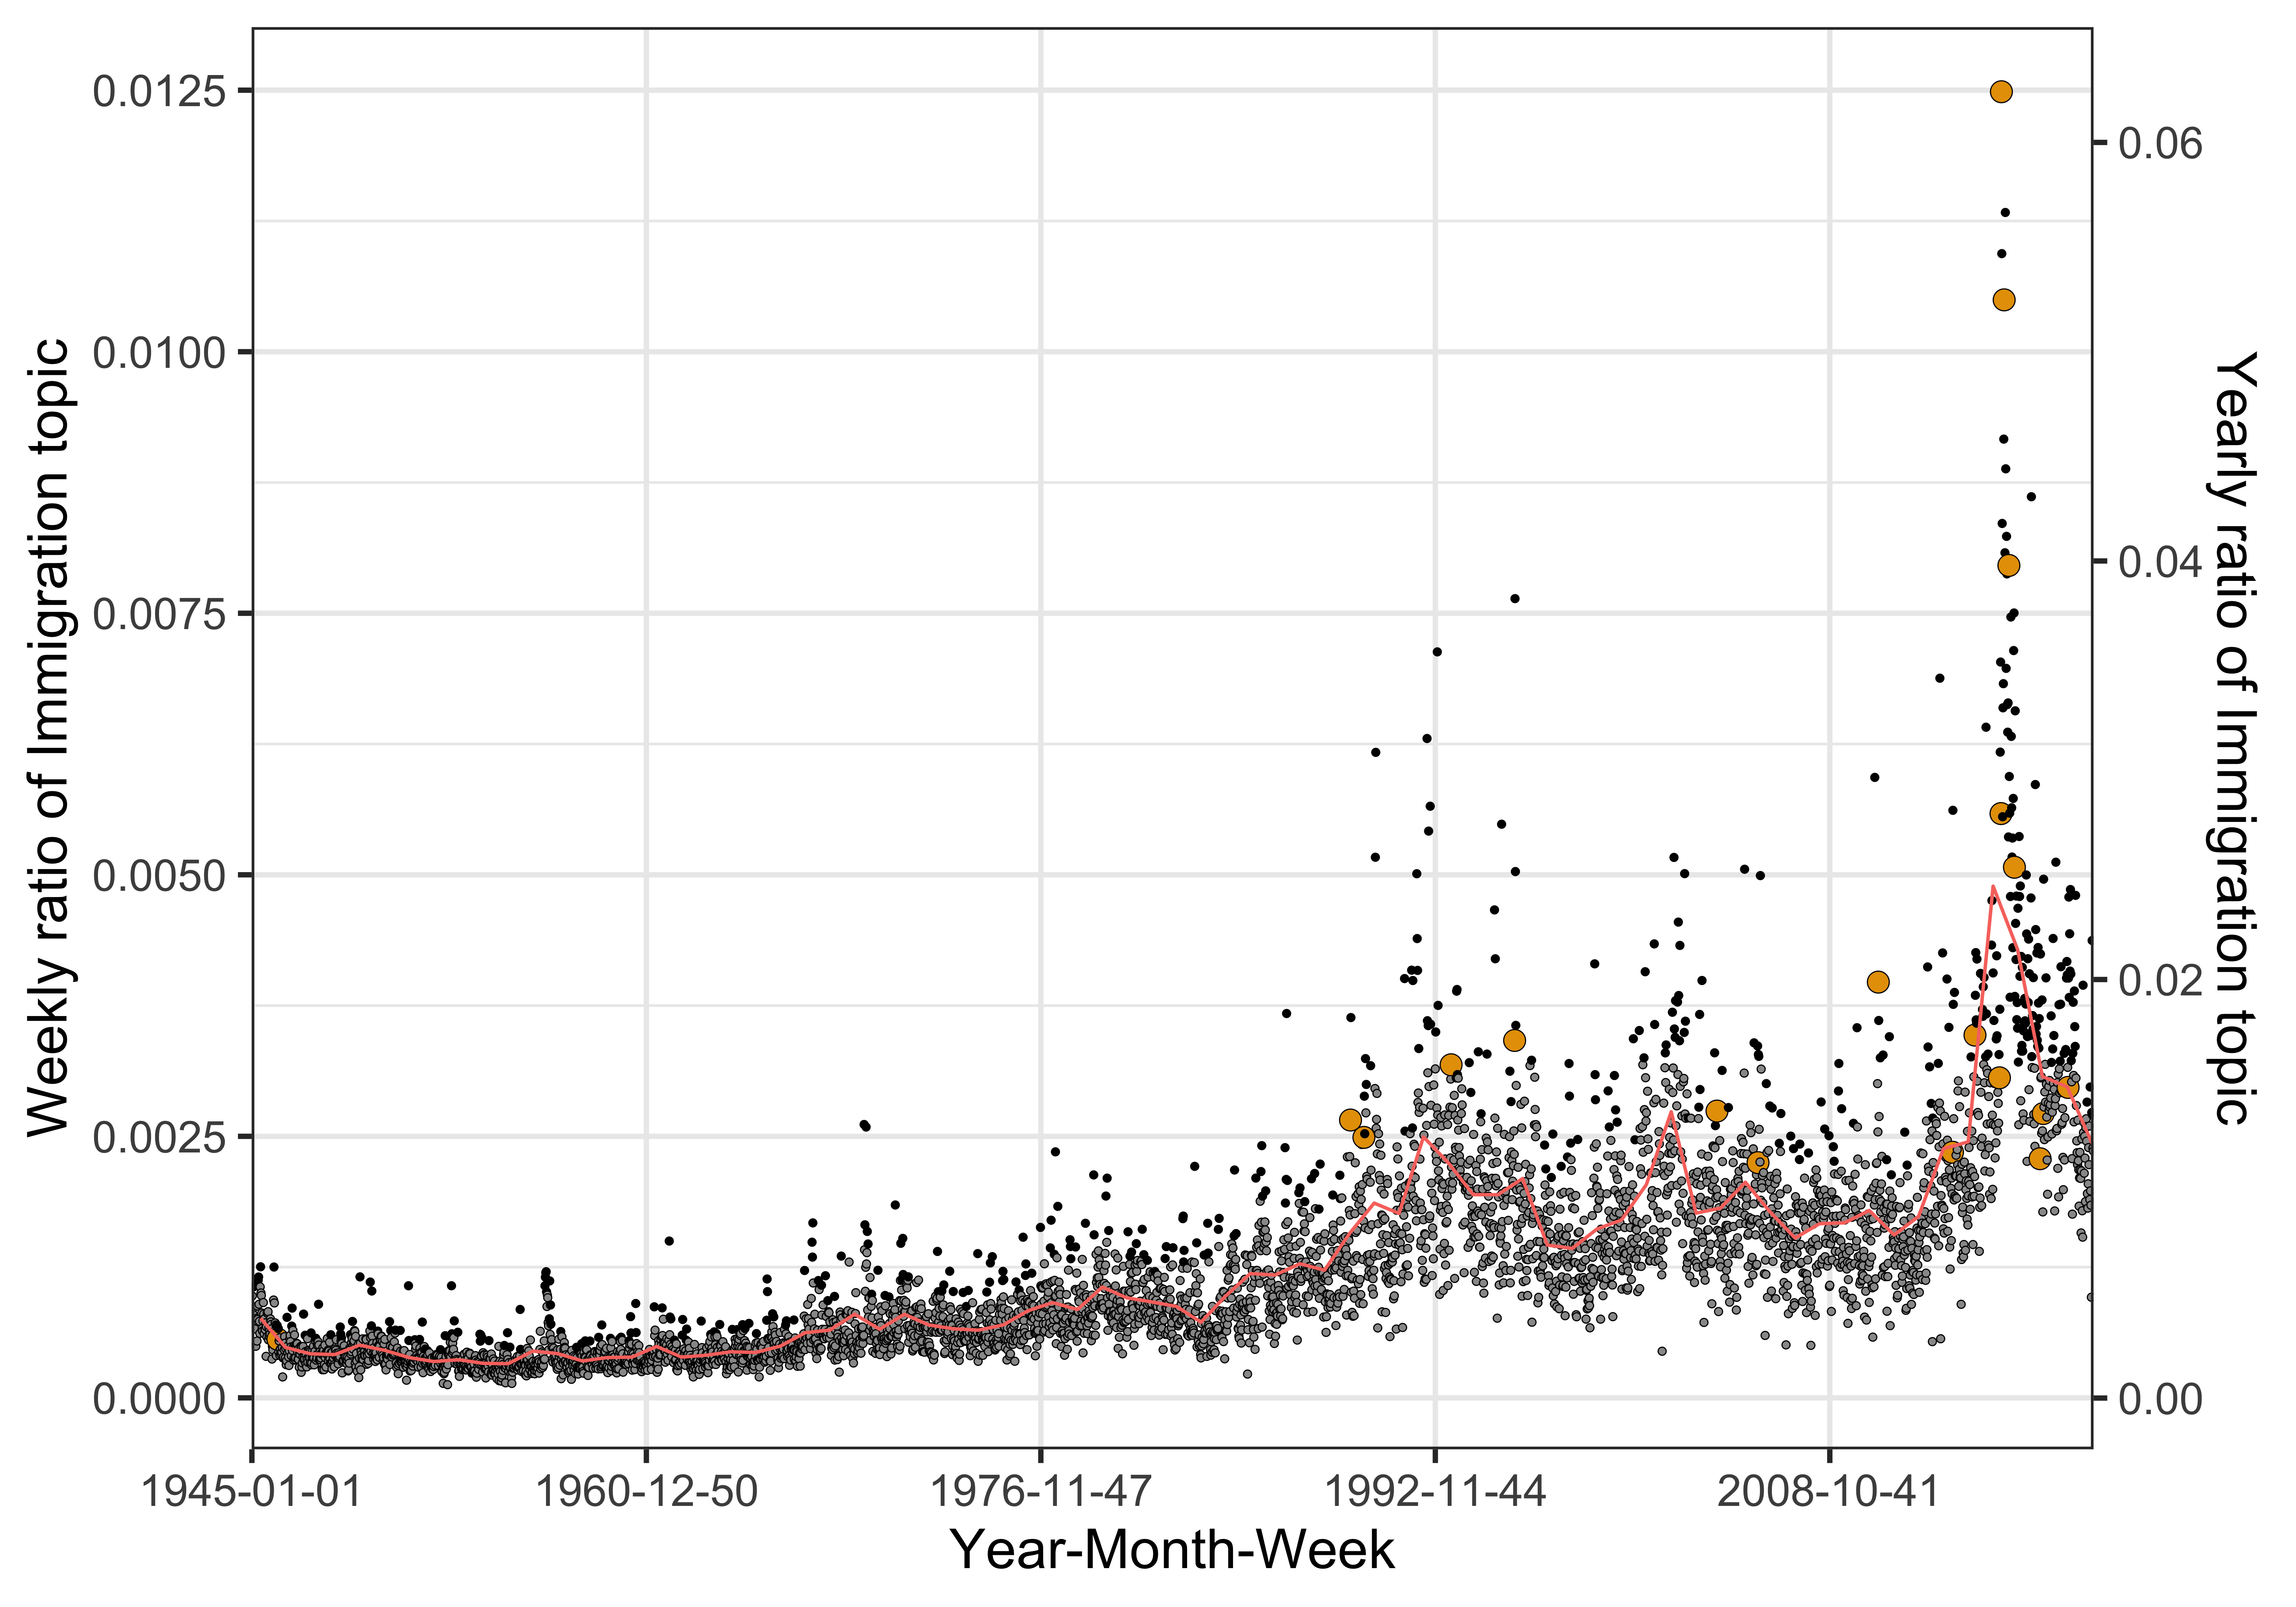
\includegraphics[width=0.9\textwidth]{fig/weekly_yearly_tot_outliers.png}
\caption{The Immigration topic in Swedish Newspapers (Hurtado Bodell et al, not in print)}
\end{center}
\end{figure}

\end{frame}


\begin{frame}{Summary: Topic Models}

\begin{itemize}
    \item Topic models are unsupervised methods for textual data\pause
    \item The Latent Dirichlet Allocation is a popular model\pause
    \item A mixed membership model (a mixture of multinomial mixtures model)\pause
    \item Usually use Gibbs samplers for estimation
\end{itemize}
\end{frame}

\end{document}
